\documentclass[a4paper,11pt,notitlepage,fullpage]{article}
%\documentclass{report}

\usepackage{fullpage}
\usepackage[utf8]{inputenc}
\usepackage[ngerman]{babel}
%\usepackage[english]{babel}
\usepackage{amsmath}
\usepackage{amssymb}
\usepackage{latexsym}
\usepackage{mathtools}
\usepackage{listings}
\usepackage{algorithm}
\usepackage{algpseudocode}
\usepackage{graphicx}
\usepackage{booktabs}
\usepackage{hhline}
\usepackage{amsthm}
\usepackage{cite}
\usepackage{wrapfig}
\usepackage{hyperref}
\usepackage{titling}
\usepackage{color}

\setlength{\droptitle}{-60pt}

\newcommand{\R}{\mathbb R}

\begin{document}
\author{Florian Bogner \& Alexander Palmrich}
\title{Stochastische Prozesse - Übung 3}
\maketitle

\begin{enumerate}
\setcounter{enumi}{10}

%11
\item bla

%12
\item bla

%13
\item bla

%14
\item
\begin{enumerate}
\item $Z = 1_{[1, 2)} W(1) + 1_{[2, 3)} W(2)$ ist eine Treppenfunktion mit 2 Treppen. Man beachte, die vermeintlich erste Treppe ist immer 0, da für $0 \leq t < 1$ gilt $W(\lfloor t\rfloor) = W(0) = 0$.
\begin{figure}[h!]
\centering
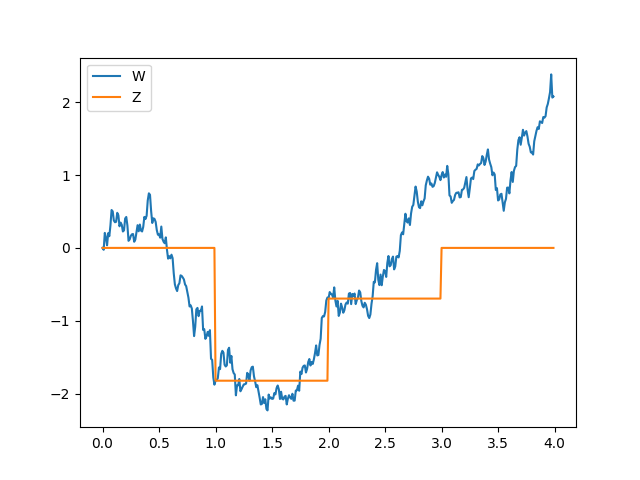
\includegraphics[width=0.66\textwidth]{gfx/14_fig.png}
\caption{Ein typischer Pfad von $W$ und $Z$}
\end{figure}

\item Messbarkeitsbedingung: Der Funktionswert $\eta_j$ muss $\mathcal F(t_j)$-messbar sein, i.e. zu Beginn des Intervalls schon bekannt sein. Dies ist der Fall, da der Funktionswert ja der Wert des Wienerprozesses zu Beginn des Intervalls ist.

Integrabilitätsbedingung: $\infty \stackrel{!}{>} E[\eta_j^2] = E[W(t_j)^2] = V[W(t_j)] = t_j < \infty$

\item Stochastisches Integral für $M_{step}^2$:
\begin{align*}
Y(t) &= \int_0^t Z(s)dW(s) \\
Y(2) &= W(1) \cdot (W(2) - W(1)) \\
Y(3) &= W(1) \cdot (W(2) - W(1)) + W(2) \cdot (W(3) - W(2))
\end{align*}

\item Mit Baby-Itô-Isometrie:
\begin{align*}
E\left[Y(3)^2\right] &= E\left[\int_0^3 Z(s)^2 ~ds\right] \\
&= E\left[\int_0^3 1_{[1, 2)} W(1)^2 + 1_{[2, 3)} W(2)^2 ~ds\right] \\
&= E\left[W(1)^2 + W(2)^2\right] \\
&= 1 + 2 = 3 \\
\end{align*}

\end{enumerate}


%15
\item Angenommen $W$ ist eine Brownsche Bewegung und $f: \R_+ \to \R$ ist eine beschränkte stetige Funktion und $0 \leq t_0 < t_1 < \cdots < t_n$. Welche Verteilung hat die Zufallsvariable
\begin{align*}
U = \sum_{k=1}^n f(t_{k-1})\Delta W(t_k)
\end{align*}
Die vorkommenden Inkremente von $W$ sind bekanntlich unabhängig normalverteilt, i.e. $\Delta W(t_k) \sim N(0, t_k - t_{k-1})$. Demnach ist $U$ eine Linearkombination aus Normalverteilungen und nach dem Reproduktionssatz wieder eine Normalverteilung. Mit
\begin{align*}
A &:= (f(t_0), f(t_1), \cdots, f(t_{n-1}) \in \R^{1\times n} \\
\mu &:= (0, 0, \cdots, 0)^T \in R^n \\
\sigma &:= diag(t_1 - t_0, t_2 - t_1, \cdots, t_n - t_{n-1}) \in \R^{n\times n}
\end{align*}
folgt:
\begin{align*}
U &\sim N\left(A\mu, A^T \sigma A\right) \\
&\sim N\left(0, \sum_{k=1}^n f(t_{k-1})^2(t_k - t_{k-1})\right)
\end{align*}
Erwartungswert und Varianz stehen damit schon da.


\end{enumerate}












\end{document}